\documentclass{article}

\usepackage{graphicx}
\usepackage{tikz}
\usepackage{tikzsymbols}
\usetikzlibrary{calc,patterns,shapes.geometric}
\pagestyle{empty}
\usepackage[margin=0pt]{geometry}
\geometry{papersize={14in,12in}}

\def\centerarc[#1](#2)(#3:#4:#5){\draw[#1] ($(#2)+({#5*cos(#3)},{#5*sin(#3)})$) arc (#3:#4:#5);}

\begin{document}
	\begin{figure}
		\centering
		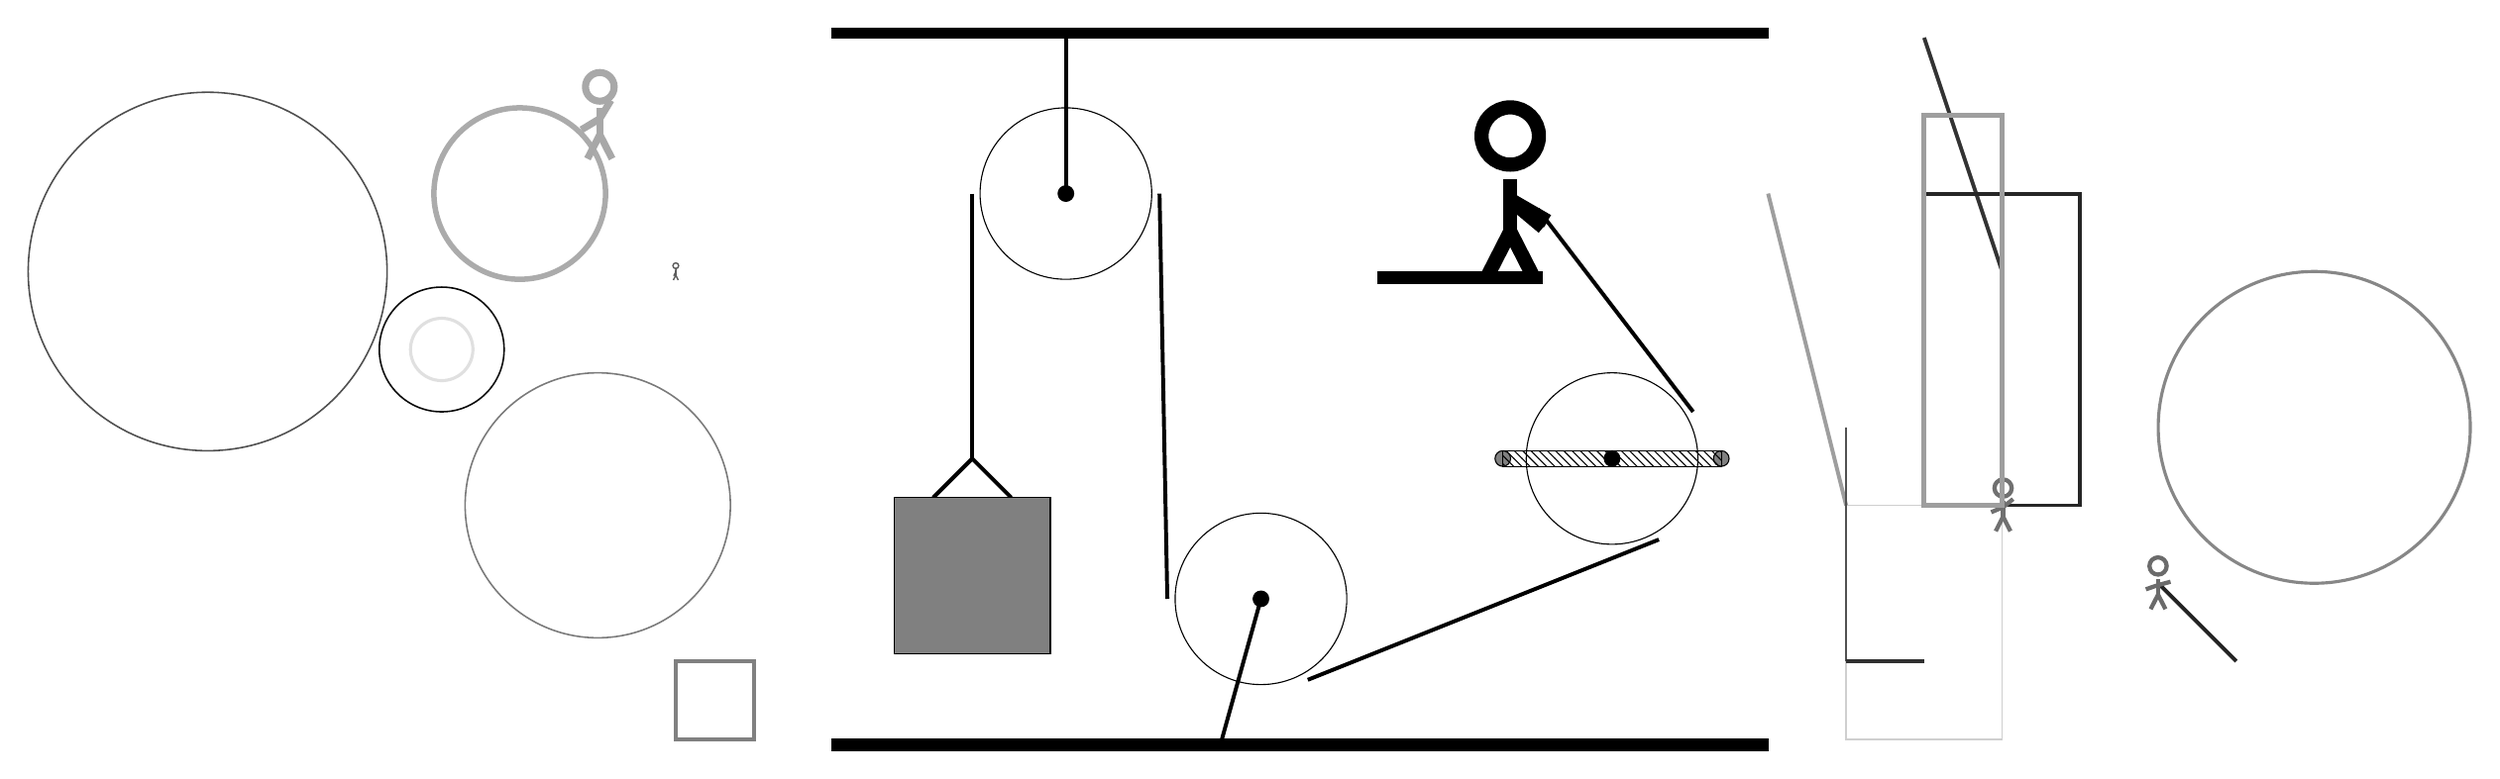
\begin{tikzpicture}
			%%%%% START %%%%%
			
			\draw[fill=black] (-2, 9) rectangle (10, 9.125);
			
			\draw (1, 7) circle (1.1);
			\draw[fill=black] (1, 7) circle (0.1);
			\draw[line width=0.5mm] (1, 9) -- (1, 7);
			
			\draw (3.5, 1.8) circle (1.1);
			\draw[fill=black] (3.5, 1.8) circle (0.1);
			\draw[line width=0.5mm] (3.5, 1.8) -- (3.0, 0);
			
			\draw[fill=white](8, 3.6) circle (1.1);
			\draw[fill=black] (8, 3.6) circle (0.1);
			\draw[fill=black!50] (9.4, 3.6) circle (0.1);
			\draw[fill=black!50] (6.6, 3.6) circle (0.1);
			\draw[pattern=north west lines, pattern color=black] (6.6, 3.7) rectangle (9.4, 3.5);
			
			\draw[line width=0.5mm](-0.7, 3.1) --  (-0.2, 3.6) -- (0.3, 3.1);
			\draw[fill=black!50] (-1.2, 3.1) rectangle (0.8, 1.1);
			
			\draw[line width=0.5mm](-0.2, 7) -- (-0.2, 3.6);
			\centerarc[line width=0.5mm](1, 7)(180:0:1.2000000000000002)
			\draw[line width=0.5mm](2.2, 7) -- (2.3, 1.8);
			\centerarc[line width=0.5mm](3.5, 1.8)(180:300:1.2000000000000002);
			\draw[line width=0.5mm](4.1, 0.7608) -- (8.6, 2.5608);
			\centerarc[line width=0.5mm](8, 3.6)(300:390:1.2000000000000002);
			\draw[line width=0.5mm](9.0392, 4.2) -- (7.05, 6.8);
			
			\draw[line width=0.5mm, color=black!80](12, 9) -- (13, 6);
			
			\draw[line width=0.6mm, color=black!96] (10, 6) rectangle (10, 6);
			\draw[line width=0.5mm, color=black!85] (12, 7) rectangle (14, 3);
			\draw [line width=0.7mm, color=black!33](-6, 7) circle (1.1);
			\draw[line width=0.5mm, color=black!50] (-3, 1) rectangle (-4, 0);
			\draw [line width=0.4mm, color=black!47](17, 4) circle (2.0);
			\draw [line width=0.4mm, color=black!12](-7, 5) circle (0.4);
			\draw[line width=0.2mm, color=black!19] (11, 0) rectangle (13, 3);
			\draw [line width=0.2mm, color=black!69](-10, 6) circle (2.3);
			\draw[line width=0.5mm, color=black!38](11, 3) -- (10, 7);
			
			\draw[line width=0.5mm, color=black!86](15, 2) -- (16, 1);
			
			\node[line width=0.6mm, color=black!34] at (-5, 8) {\Strichmaxerl[5][31][59]};
			\node[line width=0.4mm, color=black!58] at (15, 2) {\Strichmaxerl[3][19][15]};
			
			\node[line width=0.5mm, color=black!56] at (13, 3) {\Strichmaxerl[3][23][39]};
			\draw[line width=0.3mm, color=black!68] (11, 4) rectangle (11, 1);
			\draw[line width=0.6mm, color=black!38] (12, 8) rectangle (13, 3);
			
			\draw [line width=0.2mm, color=black!97](-7, 5) circle (0.8);
			\node[line width=0.5mm, color=black!64] at (-4, 6) {\Strichmaxerl[1][61][86]};
			\draw[line width=0.5mm, color=black!81](11, 1) -- (12, 1);
			
			\draw [line width=0.2mm, color=black!52](-5, 3) circle (1.7);
			
			\node at (6.75, 7) {\Strichmaxerl[10][-220][-30]};
			\draw[fill=black] (5, 6) rectangle (7.1, 5.85);
			
			\draw[fill=black] (-2, 0) rectangle (10, -0.15);
			
			%%%%% END %%%%%
		\end{tikzpicture}
	\end{figure}	
\end{document}